\section{A camera without a lens}\label{sec:no-lens}

\begin{quote}
\textbf{In plain words.} A glass lens works because glass slows light. Nothing
slows, bends or blocks gravitational waves enough to matter, so this camera
can have no lens, no mirror and no shutter. It does not need them. Each pixel
records the wave itself, crest by crest, and a computer can then combine the
pixels to do what a lens would have done.
\end{quote}

\paragraph{Nothing to build optics from.} Matter of density $\rho$ changes the
speed of a gravitational wave of angular frequency $\omega$ by the fraction
\cite{Peters1974}
\begin{equation}\label{eq:index}
n - 1 = \frac{2\pi G \rho}{\omega^{2}} ,
\end{equation}
which for steel at $1\,\mathrm{kHz}$ is $10^{-13}$, and falls as the square of
the frequency. A steel lens a metre thick would bring such a wave to a focus
only some $10^{13}$ metres away, beyond the orbit of Pluto; and since the wave
is three hundred kilometres long, a lens able to act on it at all would have
to be far larger. The same number sets reflection: by our estimate a steel
wall, however thick, returns less than $10^{-27}$ of the energy of a kilohertz
wave. Absorption is weaker still
(Section~\ref{sec:thermal}).

A mass does bend passing waves by its gravity, exactly as it bends light, by
the angle $4GM/bc^{2}$ for a ray passing at distance $b$. Used as a lens, the
Earth has a focal length of fifteen thousand times the distance to the Sun,
and a focal ratio near $10^{8}$. In each case the strength of the effect is
set by the same number, the compactness $GM/Rc^{2}$ of the body, which is
$7\times10^{-10}$ for the Earth and of order one only for a black hole. Bounds
of this kind on absorption are known \cite{Loeb2020}. We expect a single
statement to cover all four effects: no body much less compact than a black
hole can focus, reflect, absorb or block gravitational waves appreciably.
Proving it is part of this work. In the gravitational sky, only black holes
cast shadows.

\paragraph{The computed image.} The camera does not need optics, because its
pixels record more than a light sensor does. A light sensor registers only
the energy that arrives. A gravitational pixel registers the field itself,
with its phase. Waves from a direction $\hat n$ reach different pixels at
different times, and the image is made by undoing those delays and adding:
\begin{equation}\label{eq:beam}
I(\hat n) = \Bigl\langle\, \Bigl|\, \sum_{p} \tE\bigl(\mathbf{x}_p,\;
t + \hat n\cdot\mathbf{x}_p/c\bigr) \Bigr|^{2} \Bigr\rangle ,
\end{equation}
where $\mathbf{x}_p$ is the position of pixel $p$. Waves from the chosen
direction add in step; waves from elsewhere cancel. This is how arrays of
radio telescopes form images, and it is what a lens does with glass. The
sharpness is that of any aperture of width $D$,
\begin{equation}\label{eq:diffraction}
\Delta\theta \approx \frac{\lambda}{D} ,
\end{equation}
shown in Figure~\ref{fig:array}. In the near field there are no delays to
undo, and the image is instead obtained by the inversion of
Section~\ref{sec:near-field}.

\begin{figure}
\centering
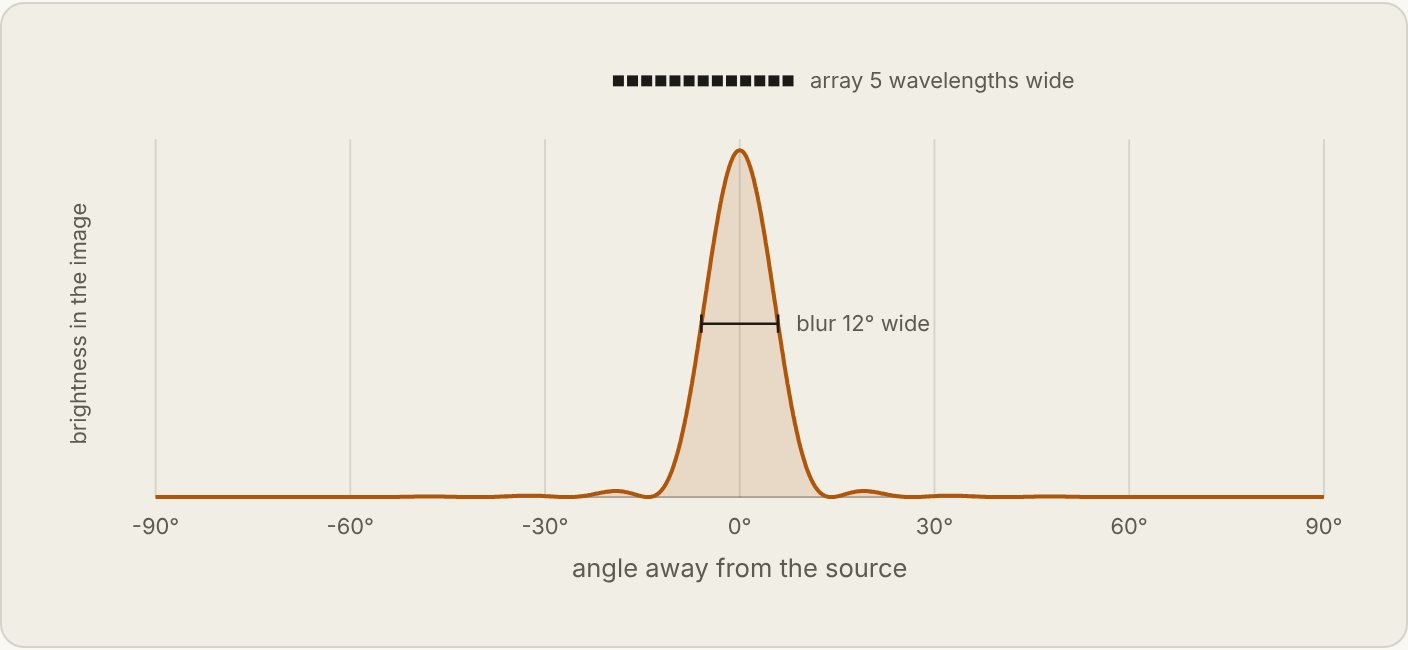
\includegraphics[width=\linewidth]{figures/array.png}
\caption{How sharply a camera can tell directions apart. The curve is the
response to a single distant source as the computed image is steered away from
it. A single pixel is not blind to direction, but its view of the sky is
blurred over tens of degrees. An array sharpens in proportion to its width in
wavelengths, Eq.~\eqref{eq:diffraction}.}\label{fig:array}
\end{figure}

\paragraph{What one pixel knows.} A single LIGO cannot tell where a wave came
from. A single ideal pixel can do better, because it records all ten
components of the field. For a single wave, the tensors $\tE_{ij}$ and
$\tB_{ij}$ together fix the direction of travel. For a sky full of independent
sources the pixel's data determine the brightness of the sky only in its
broadest patterns: those of spherical-harmonic degree four or less,
twenty-five numbers in all. It is the gravitational counterpart of the
statement that a single antenna has a broad beam, and it is the precise sense
in which one pixel is not yet a camera.

The proof is short. Independent waves add their second moments, so the
pixel's data are integrals over the sky of the brightness $I(\hat n)$ and the
circular polarization $V(\hat n)$ against kernels made from the polarization
tensors of a plane wave travelling along $\hat n$. For the brightness the
kernel is the sum over the two polarizations,
\begin{equation}\label{eq:pixel-kernel}
\sum_{A=+,\times} e^{A}_{ij}\, e^{A}_{kl}
= P_{ik}P_{jl} + P_{il}P_{jk} - P_{ij}P_{kl},
\qquad P_{ij} = \delta_{ij} - \hat n_i \hat n_j ,
\end{equation}
a polynomial of degree four in the components of $\hat n$; the kernel for $V$
is the antisymmetric combination, also a polynomial of degree at most four.
A polynomial of degree four on the sphere contains spherical harmonics of
degree four and below only, so by their orthogonality every harmonic of $I$
and $V$ above degree four integrates to zero. The magnetic tensor of a plane
wave is the electric one turned by $45^\circ$ about $\hat n$, so the same
holds for every product of $\tE$ and $\tB$. The linear polarization carries
spin weight four about $\hat n$ and enters only through its harmonic of degree
exactly four. The reference implementation checks all three statements
numerically, harmonic by harmonic.
